\section{Quantifying Baryon Redistribution}
\label{sec:feedbackmetrics}

Feedback is a complex process that impacts a wide range of
baryonic observables, from the galaxy stellar mass function, to galaxy sizes,
to the density profiles of galaxies \citep[e.g.][]{BenitezLlambay2018}. It is
interesting, therefore, to develop tools to study the global effects of
feedback directly, as a complement to the many indirect constraints
obtainable from comparing to astrophysical observables. Here we describe the
tools we will use to examine the redistribution of baryons via feedback.

The kinetic feedback scheme used in \simba{} for both star formation and AGN
feedback makes it straightforward to identify the gas elements that have been
directly impacted by feedback. However, these gas elements will then go on to
entrain and deposit energy into other gas elements as they travel. This makes
it challenging to fully capture the impact of feedback solely from particle
tagging. Another option to assess feedback is to run simulations with
specific feedback modules turned on and off. However, this is inconsistent
with the tuning procedure that virtually every simulation suite performs in
order to constrain the many parameters in the sub-grid model. For instance,
modern models are typically calibrated to the $z=0$ Stellar Mass Function
(SMF), which will of course change should some feedback mechanism be missing
(and hence should be re-calibrated). It is thus important to realize that, if
without some feedback module a simulation fails to match data, this does not
definitively prove that the feedback module is necessary to produce realistic
galaxies, since it could potentially be that the simulation could be
recalibrated to match data in some other way. In our case, we run the \nojet{}
and non-radiative variants in order to explore how baryon redistribution is
sensitive to these feedback modules, but we do not attempt to recalibrate
these to data, and merely use them in order to investigate the impact of this
input physics within the context of the \simba{} model.

\subsection{The Spread Metric}

\begin{figure}
    \centering
    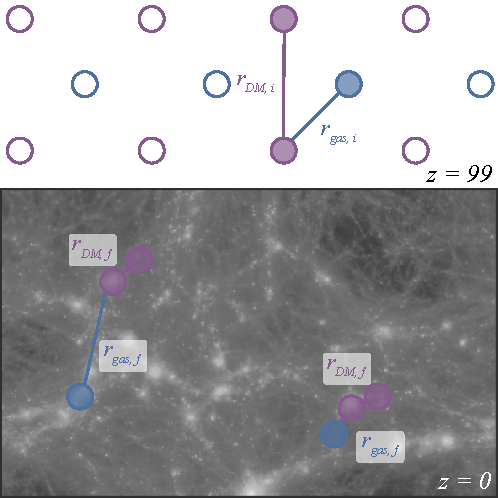
\includegraphics[width=\columnwidth]{figures/kspafig_small.pdf}
    \vspace{-0.5cm}
    \caption{Illustration of the matching procedure between initial and final conditions to define the spread metric. The top panel shows the $z=99$ initial conditions, where
    every particle finds its nearest dark matter neighbour. The bottom
    panel shows the distances between those particles at $z=0$. For our
    fiducial results, each particle is matched to the three nearest 
    neighbours at $z=99$ and the spread metric is computed as the median 
    of the corresponding distances at $z=0$ (see text for details). 
    %but this is omitted in this simple picture for brevity.
    }
    \vspace{-0.5cm}
    \label{fig:kspafigsmall}
\end{figure}

Our approach to quantifying the large-scale impact of feedback is to develop
a simple and robust metric that directly captures the displacement of gas
owing to feedback. This `spread' metric, illustrated in Figure
\ref{fig:kspafigsmall}, works as follows:

\begin{enumerate} 
	\item For every gas particle $i$ in the initial conditions, find the nearest
          $n$ dark matter neighbours $j$ (with $n=3$ for our fiducial results).
	\item In the final conditions at $z=0$, match all remaining baryonic particles
	      with their initial conditions progenitor (in this case, stars are
	      matched with their gas particle progenitor).
	\item Find the distance $r_{ij}$ in the final conditions, i.e. the distance between particle $i$ and its original neighbours. 
	\item The spread metric for particle $i$, denoted $S_{n}^{i}$ [or maybe $S_{D}^i$ or maybe $D_{s}^i$ or maybe $S_i$...], is given by the \emph{median} of the $n$
	      original dark matter neighbour distances $r_{ij}$.
\end{enumerate}

\begin{figure}
    \centering
    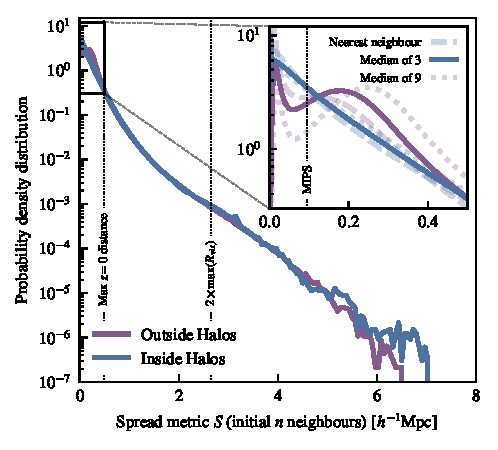
\includegraphics{figures/s50j7kAHF/dark_matter_distance_figure_s50j7k_AHF}
    \vspace{-0.5cm}
    \caption{%The distribution of final-state distances from the spread metric for dark matter
    Distribution of spread metric distances at $z=0$ for the dark matter component 
     in the full \simba{} model. 
    %This distribution is relatively unchanged by the choice of sub-grid model, and the effects of     the back-reaction of baryonic physics on dark matter is out of the scope of this work. 
    The distribution is split between particles that lie within halos (blue) and outside halos (purple), with this being an approximately even
    split at $z=0$. Vertical dotted lines indicate the maximal distance
    between any two dark matter particles at $z=0$ ( 
    $\sim 0.5\hmpc{}$) and twice the maximal virial radius of any halo in the box ($R_{\rm vir}^{\rm max} \sim 1.3\hmpc{}$). 
    The inset figure shows the inner
    $0.5\hmpc{}$ of the distribution, 
    %and has a line over-plotted for the
    with the mean inter-particle separation in the initial conditions (MIPS $\sim 0.1\hmpc$) indicated by the vertical dotted line. The fainter lines show how the spread
    metric changes when taking the median over a different number of initial
    nearest neighbours.
    %[DAA: I think we can skip this]; dashed gives the metric with no median (i.e. only one nearest neighbour), and the dotted line shows the case for a median over 9 neighbours. 
    }
    \vspace{-0.5cm}
    \label{fig:dmonlyspread}
\end{figure}

The `spread' metric is presented first for dark matter in Figure
\ref{fig:dmonlyspread}. The simplest metric here clearly is simply to use the
nearest neighbour in the initial conditions, rather than the median over $n$
initial neighbours. The choice of $n=3$ was made primarily to ensure that the
dark matter results were robust when comparing matter inside and outside of
halos. For a given dark matter particle pairing, a large distance between two
neighbours would be `double counted' for the case where one neighbour makes
it into a halo and one remains outside, contributing the large distances to
both bins. Choosing $n=3$ enables the median result to represent the distance
to a real particle, and removes the problem of double counting for the
nearest neighbour. The overall distributions of distances were not changed
much by this choice, however larger choices for $n$ increase the contrast in
the dark matter images in Figure \ref{fig:bigdistanceimage}, with more
substructure picked up in the low-spread particles, and show more diffuse
structure in the high-spread particles.

\subsection{Baryon Spreading in \simba{}}

Figure \ref{fig:distbaryon} shows how the distribution of spread distances
for the gas particles is significantly different to that for the dark matter.
Gas particles are able to spread to much larger distances, up to $12\hmpc{}$,
compared to the $7\hmpc{}$ that dark matter can reach. We also see that even halo gas is spread more than the dark matter, when explicitly selecting for this
component.

Another interesting 
%selection to make 
component is the gas that originated in
Lagrangian regions (i.e. next to the dark matter that will reside in halos at $z=0$), indicated by the blue dashed line. With the baryon fraction of halos being typically less than $50\%$ of
the cosmic mean, we should expect that a 
%lot of this gas is lost over time,
significant amount of Lagrangian gas is lost over time, possibly spreading to large distances out of halos owing to 
%. This gas may also be expelled from the halos in
high energy feedback events, either through galactic winds or AGN feedback. In \simba{}, we see that gas from Lagrangian regions indeed spreads systematically
further, 
%with there being approximately a factor of two 
with a factor of $\sim 2$ more particles at
distances larger than $\sim 4 \hmpc{}$ than an unbiased selection would
suggest.

\begin{figure}
    \centering
    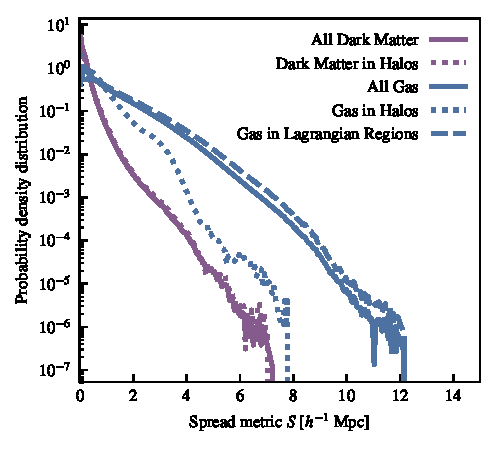
\includegraphics{figures/s50j7kAHF/distance_plot_split_by_component+AHF.pdf}
    \vspace{-0.5cm}
    \caption{Spread distance distribution for gas at $z=0$ (blue) compared to that of the dark matter component (purple).  Solid lines indicate the full distribution, dotted lines correspond to gas/dark matter inside $z=0$ halos, and the blue dashed line shows the distribution for gas inside of Lagrangian regions at $z=99$.   
    Note how, compared to the dark matter, the distributions for gas inside
    halos and outside halos are significantly different, with gas that
    originated in lagrangian regions being preferentially moved to larger
    distances than gas on average. Note that only 10\% of the gas in the
    entire simulation is in halos at $z=0$. Gas can be blown out to
    $12\hmpc{}$, approximately 10 times the virial radius of the largest halo
    in the box.}
    \vspace{-0.5cm}
    \label{fig:distbaryon}
\end{figure}

\begin{figure*}
    \centering
    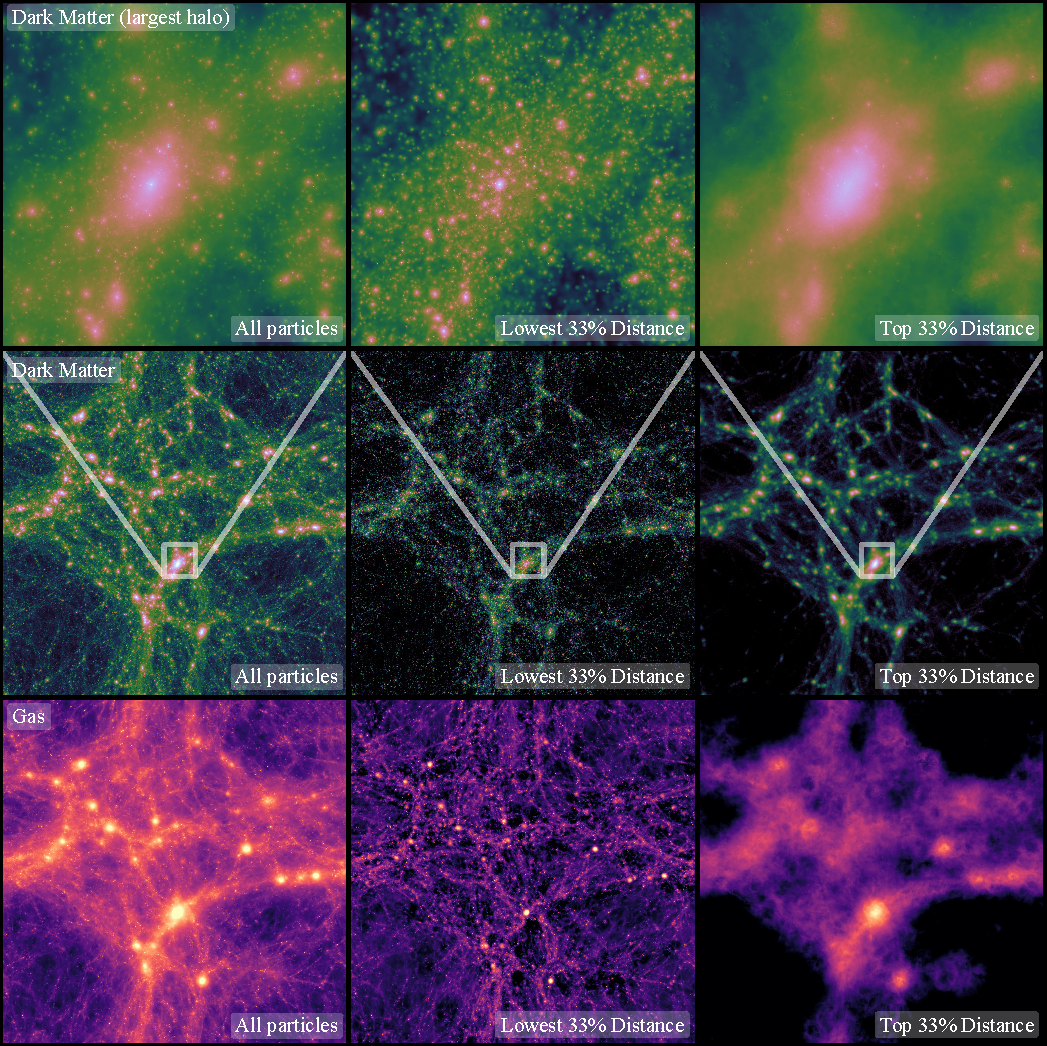
\includegraphics[width=\textwidth]{figures/distance_figures_3.pdf}
    \caption{Projected mass surface density distributions for different particle selections at $z=0$.
    The three rows show, 
    %the following selections of particles, 
    from top to bottom, the dark matter in a $4.5\hmpc{}$ cubic volume centred around the largest halo ($R_{\rm vir}\sim 1.3\hmpc{}$)
    %present in the largest halo, and surrounding it (this is a $4.5\hmpc{}$ cube centred around the halo centre, which has a virial radius of approximately $1.3\hmpc{}$)
    and the dark matter and gas distributions in the $50\hmpc{}$ box.
    %; and the gas distribution in the box. 
    %All images are shown in the final state of the simulation at redshift $z=0$. 
    Columns show, from left to right, all
    particles inside of the corresponding volume, the 33\% of the particles with the lowest spread distance, 
    %selecting the lowest 33\% from the histogram figures
    and the 33\% of the particles that have spread the  most. For the dark matter, these cuts
    correspond to particles that have travelled less than $0.1\hmpc{}$ and
    more than $0.25\hmpc{}$, respectively. For the gas, these numbers
    increase to $0.45\hmpc{}$ and $1.25\hmpc{}$, respectively, due to the
    larger spread that gas particles experience. 
    Each density projection is generated using smoothing
    lengths defined to encompass the $32$ nearest neighbours
    %[DAA: Simba uses 64 ngbs actually], as is used in the \simba{} simulations, 
    and smoothing lengths are kept consistent across
    columns (i.e. they are not recomputed for different particle distributions). All density projections in a given row also
    use the exact same (logarithmic) normalisation and colour map to enable direct
    comparisons. Note 
    %how even with this extremely conservative cut there is a significant difference between the images, with sub-structure picked out by the low-distance cut and large-scale structure for the large-distance cut.
    the significant difference between the spatial distribution of material with different spread metric, with sub-structure preferentially picked out by the low spread distance selection while the large spreads trace large scale structure.
    }
    \vspace{1cm}
    \label{fig:bigdistanceimage}
\end{figure*}

These significantly different spread distributions of gas and dark matter should correspond to
significantly different spatial distributions. In the below we define
`low-spread' particles as those in the lower tertile (33\%) of the
distribution, and `high-spread' particles as those that are in highest
tertile of the distribution.

A visualisation of the low- and high-spread particles is shown in Figure
\ref{fig:bigdistanceimage} for both dark matter and gas, for the fiducial
\simba{} model. By making (generous) cuts in the distance distribution, we
are able to show that the low-spread particles correspond to substructure,
with the high-spread particles contribution being the larger-scale, more
diffuse, CGM and IGM.

Considering first the dark matter in the largest halo (top row),
we see that the very small-scale substructure of the halo is preferentially picked up by the low-spread particles, including the central
density peak itself and the centers of subhalos. In contrast, the more diffuse dark matter component that fills the space between these individual
density peaks is significantly more prominent in the high-spread particles, with only a small
amount of residual sub-structure remaining. These trends are also clear at larger scales, as shown by the view of the $50\hmpc{}$ box in the second row, with large-scale dark matter
filaments primarily traced by high-spread particles. It is interesting to note that
a large amount of structure in voids is not present in either of these
panels, with it being captured by the medium-spread particles with values $0.1\hmpc{} < S_{n}^{i} < 0.25 \hmpc{}$. The spread metric is thus a very useful tool to connect hierarchical structure and dynamical evolution in cosmological N-body simulations.

The bottom row in Figure~\ref{fig:bigdistanceimage} shows the large scale gas distributions separated with the same proportions, with $1/3$ of the total gas mass contained in each of the middle and right panels (however, note that this corresponds to different absolute values of the spread metric compared to the dark matter panels). The low-spread particles trace the densest gas in halos
%cores of galaxies and their disks, along with some residual filamentary structure. 
along with lower density gas in the central parts of large scale filaments.
Of particular interest is the high-spread gas, which traces the large bubbles around the most massive halos that strong AGN jets produce in the \simba{} model (shown explicitly below). 
%allowing for gas that is entrained by these feedback events to be systematically identified.
As expected from Figure~\ref{fig:distbaryon}, the top 1/3 of the gas distribution has been pushed out to significantly larger distances compared to the 1/3 of the dark matter that moved the most owing to gravitational dynamics only.  The spread metric nicely captures the impact of feedback in a global sense.


\begin{figure*}
    \centering
    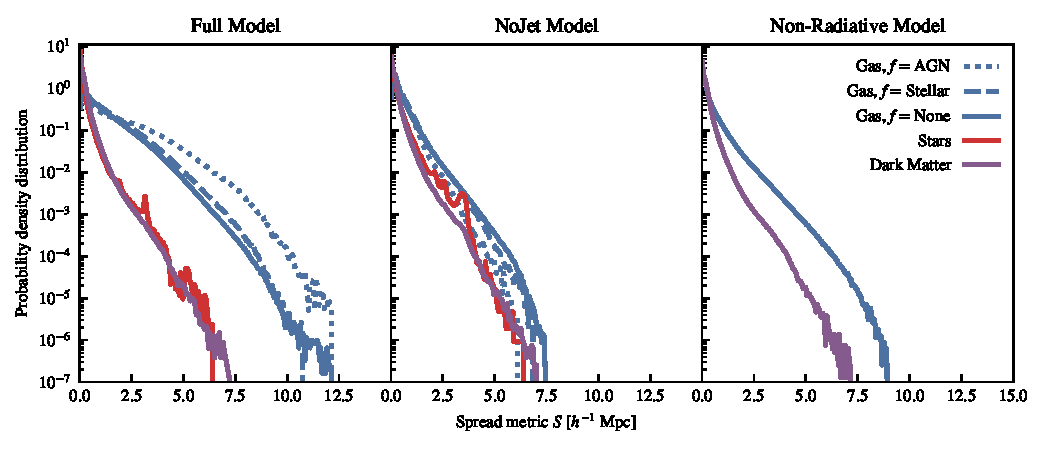
\includegraphics[width=\textwidth]{figures/neighbour_analysis_feedback_histogram_combined.pdf}
    \vspace{-0.7cm}
    \caption{Distribution of spread distances
    %for all particles $i$ to the nearest neighbour $j$ in the initial conditions, 
    split by particle type for gas (blue), stars (red), and dark matter (purple).  This is shown for the $z=0$ particle distribution in the
    reference model (left), the \nojet{} model (center), and the non-radiative simulation
    (right). The left and middle panels separate gas particles that have not been involved in any feedback event (solid) from those that have participated directly in either stellar (dashed) or AGN (dotted) feedback events. 
    %in this figure shows that the further out a particle has been blown the more likely it is to have been directly involved in a feedback event for the reference model. Also note the vertical $0.5-1$ dex offset for gas compared to dark matter even in the \nojet{} run.
    Jets are primarily responsible for spreading baryons to the largest distances in \simba{}, with significant entrainment of gas that did not directly participate in feedback events. 
    }\label{fig:feedbackdistance}
\end{figure*}

In Figure \ref{fig:feedbackdistance}, we show different models in an
attempt to better characterise the effects of different pieces of the
\simba{} sub-grid model.

The left panel, showing the full \simba{} model, splits the 
gas component into particles that have been affected by different
types of feedback. Here, AGN feedback takes precedence over stellar
feedback, such that if a particle has been affected by both it is only
classified as being part of the $f=$AGN group. We see that the particles
that have directly interacted with the AGN are spread to significantly 
larger distances, with a vertical offset of 0.5-1 dex compared to no-feedback particles 
%for a given spread metric bin at 
for $S_{n}^{i} \gtrsim 5\hmpc{}$. Particles that have been directly kicked by
stellar feedback also have systematically higher spread metric values,
albeit with a smaller offset. This implies that particles are indeed being spread to these large distances by feedback events.

The left panel also now includes the stellar component, which shows a very similar
distribution to that of dark matter. 
%despite having formed out of gas particles. 
This is expected by redshift $z=0$, as since cosmic noon at
around $z=2$ where star formation peaks, there has been many Gyrs for these
particles to virialise and relax back into equilibrium with the dark matter.
It would be unexpected for a star particle to form from a gas particle with a
high spread value, as these must have been separated dynamically from their
closest dark matter neighbour, requiring some kind of energy injection into
the gas phase. This would heat the particle, likely to a high temperature,
preventing the particle from having long enough to cool by $z=0$ to a
temperature low enough to form a star.

%The specific effect of the high-energy AGN jets is shown in [DAA: this would be more the lack of effectsince there is no jet?]
The middle panel of Figure~\ref{fig:feedbackdistance} shows the spread distribution for the \nojet{} simulation, where we still include AGN feedback in the form of radiative winds and X-ray heating but the high velocity jet feedback mode is disabled. With this change, the spread metric is 
%transformed completely,showing a much tighter correspondence between 
significantly affected, with much less difference between the distributions of
the dark matter, gas, and stellar components.
While galactic winds and AGN feedback in radiative mode can still decouple the dark matter and gas components, high-velocity jets are clearly the dominant mechanism responsible for spreading baryons to the largest distances in \simba{}.
Thanks to strong cooling flows, particles that have been directly heated by feedback (those in the densest regions) actually now show a lower spread metric than an average particle, with dark matter and gas in these dense regions unable to dynamically separate from each other.

This result is surprising given that less than $0.4\%$ of gas particles in
the simulation have ever interacted directly with the AGN jets; this has been
enough to 
%completely separate the majority of 
significantly decouple the gas from the dark matter
dynamically. Such a high degree of separation points to substantial amounts of gas
being entrained by these powerful jets. It is not simply the case that higher
mass ($M_H > 10^{11} \msolar{}$) halos are quenched internally reducing their
star formation rate; the energetics and dynamics of the CGM and IGM are
significantly altered, as is already seen by the more complex interaction
between the turn-off of the galaxy stellar mass function (GSMF) and the power
of the AGN jets in many studies.

The final contrast to highlight is the difference between the \nojet{} and
non-radiative model. The non-radiative model shows increased distance between
gas particles and their associated dark matter neighbour compared to the
\nojet{} run; this due to the lack of cooling preventing particles that lie
in small halos from remaining as tightly bound. It also highlights how
difficult it is to drive gas into the centers of structures without cooling.
The collisionless dark matter can continue to fall in to bound structures,
with the gas being prevented due to strong accretion shocks. This allows for
a very different kind of separation than what we conjectured above about the
full physics models that include cooling.

\begin{figure}
    \centering
    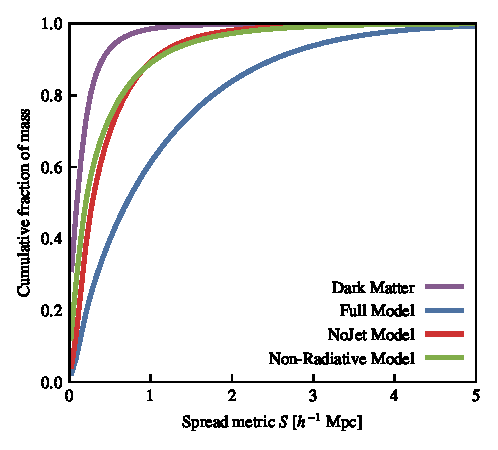
\includegraphics{figures/cumulative_histogram_comparison.pdf}
    \vspace{-0.7cm}
    \caption{Cumulative version of Fig. \ref{fig:feedbackdistance} that
    shows the gas distribution for the three models alongside the dark
    matter from the full model.}
    \label{fig:cumulativehistogram}
\end{figure}

In Fig. \ref{fig:cumulativehistogram} we show the cumulative version of Fig.
\ref{fig:feedbackdistance} to better show the amounts of mass that are spread
to large distances. The full model constrains about 90\% of the mass within
around $3\hmpc{}$, with a slow tail off ending with nearly all of the mass
being constrained to be spread less than $5\hmpc{}$.

% Placed here for organisational reasons
\begin{figure*}
	\centering
	\vspace{0.5cm}
	\includegraphics{figures/fancy-figure.pdf}
  \caption{ %[DAA: trying to simplify this a bit] This visualisation shows two epochs at once, simultaneously showing the initial conditions (in blue and red) and the final simulation volume at redshift $z=0$ in white/grey. The blue and red show the positions of the gas and dark matter (respectively) \emph{in the initial conditions} for particles that reside in selected halos at redshift $z=0$. The overlaid white/grey map shows the dark matter at redshift $z=0$ to enable comparisons between the initial and final comoving positions for various bound structures.
  Comparison between the initial and final spatial distributions of the dark matter and baryonic content of halos.
  The background grey scale shows the projected dark matter mass distribution at $z=0$ in the $50\hmpc{}$ \simba{} volume. For selected halos, we overlay the projected distribution of their dark matter content (red colour scale) and baryonic content (blue colour scale) according to their comoving location \emph{in the initial conditions} ($z=99$). The initial distribution of dark matter particles indicated in red is thus the Lagrangian region of each selected halo, with a dashed black circle indicating its virial radius at $z=0$.
  Note that the red/blue color scales are unique to each halo to enable the simultaneous visualization of all Lagrangian regions. 
  Grey circles and arrows indicate the correspondence between initial Lagrangian regions and final halos for halos with substantial peculiar motion. 
  Bar charts next to each halo indicate the fraction of their $z=0$ baryonic mass the originates from their own Lagrangian region (blue), the Lagrangian region of a different halo (red), and outside of any Lagrangian region (purple) as described below.
  %For each selected halo, the dashed black circles show their virial radii as defined in \S \ref{sec:simba}. For some halos in crowded regions, we have overlaid a circle and arrows showing which blob of dark matter and gas in the initial conditions collapses to form this halo. Finally, for each halo we show a small bar chart showing their final lagrangian make-up, as described later in the text. 
  %We recommend that readers on their first pass consider the differences in origin between the gas (blue) and dark matter (red) for these selected halos of various masses. On a second pass, stop to consider how the environment of each halo changes its lagrangian make-up. In particular, group 431 shows a large baryonic component originating from the lagrangian region of another halo, with this halo entering a small cluster environment near the end of the simulation. 
  Note the clear differences in the initial spatial distribution of the dark matter and gas that makes up each final halo.
  %Note that individual regions are colour-mapped separately, i.e. the intensity of colour for a single halo is unique to that halo only, as to enable all lagrangian regions to be seen. Without this choice, the  structure for the lower mass halos would be completely washed out.
  }
	\vspace{1cm}
	\label{fig:bigtransferpic}
\end{figure*}


\begin{figure*}
    \centering
    \vspace{1cm}
    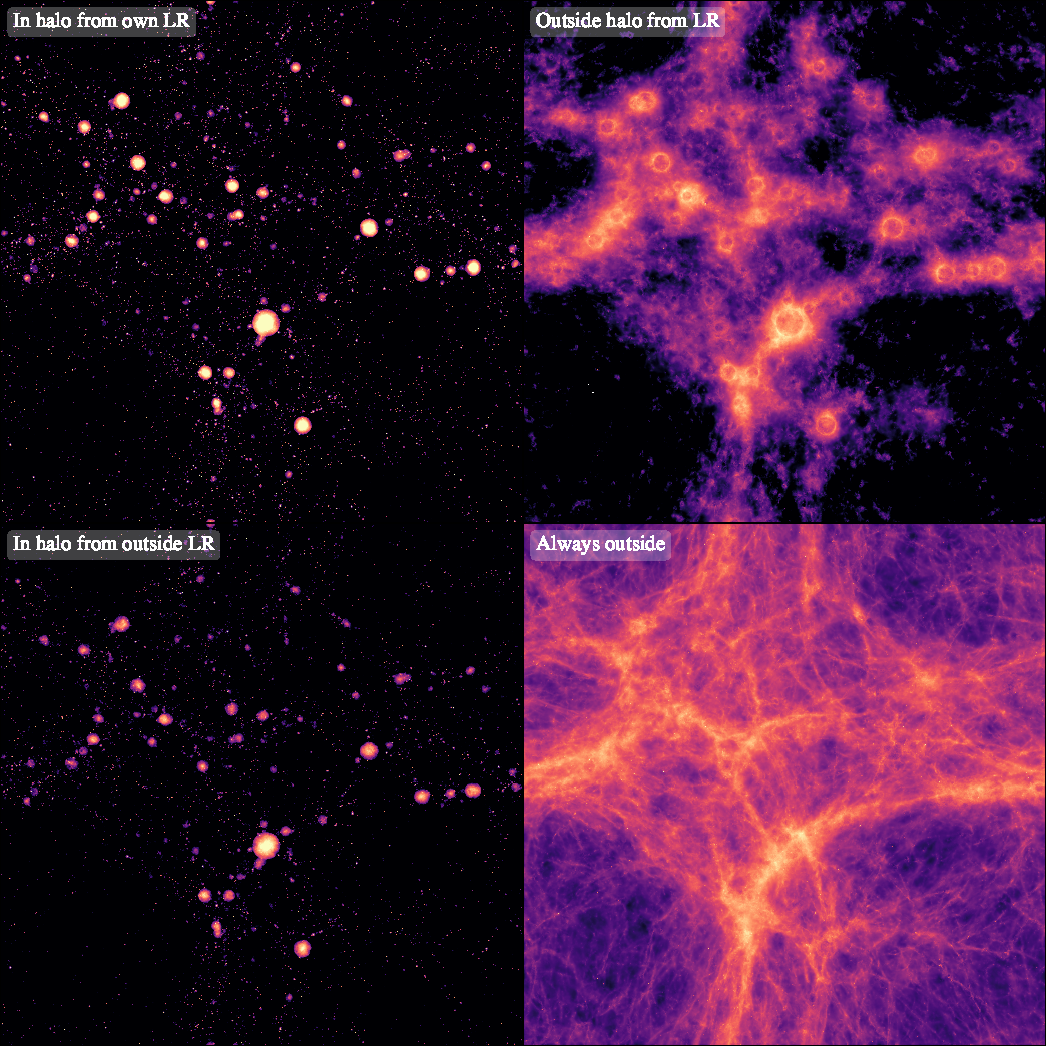
\includegraphics{figures/s50j7kAHF/four_images_magma_AHF.pdf}
    \caption{Gas distribution in the fiducial \simba{} model for the full $50\hmpc{}$ volume,
    split by the following Lagrangian components (clockwise, starting from top left): 
    particles that began in Lagrangian
    regions at $z=99$ and have remained in the associated halos at $z=0$; particles that began in Lagrangian regions and ended up outside of the destination halo;
    particles that began outside any Lagrangian region and ended up outside any halo; and particles that ended up in a halo but originated outside any Lagrangian region.
    All images are shown with the same
    (lograithmic) colour-map and normalisation and taking their linear sum
    %(ignoring the fact that the logarithmic density is plotted)
    would reproduce the full gas distribution at $z=0$.
    Gas particles that began in
    Lagrangian regions but ended up outside of halos (top right) show a striking
    similarity to the distribution of gas with the 33\% highest spread distance shown in
    Figure~\ref{fig:bigdistanceimage}. As expected, particles that began outside of Lagrangian regions and remained outside of halos (bottom right) trace the filaments and voids.}
    \vspace{1cm}
    \label{fig:lrtransfer}
\end{figure*}

These results show that gaseous and stellar matter can be transferred out to
significantly further (by $z=0$) than is assumed by typical zoom-in
simulation suites. For example, the Latte \citep{Wetzel2016} suite uses an
exclusion region for high resolution particles of around $1.5 \hmpc{}$.
Whilst they do not find contamination (possibly due to isolation criteria) of
low-resolution particles into the high-resolution region, the above metrics
suggest that perhaps this is a more numerical, rather than physical, effect;
low resolution particles are not present due to a lack of sub-grid physics in
the unrefined region.
